% mn2esample.tex
%
% v2.1 released 22nd May 2002 (G. Hutton)
%
% The mnsample.tex file has been amended to highlight
% the proper use of LaTeX2e code with the class file
% and using natbib cross-referencing. These changes
% do not reflect the original paper by A. V. Raveendran.
%
% Previous versions of this sample document were
% compatible with the LaTeX 2.09 style file mn.sty
% v1.2 released 5th September 1994 (M. Reed)
% v1.1 released 18th July 1994
% v1.0 released 28th January 1994

\documentclass[useAMS,usenatbib]{mn2e}

% If your system does not have the AMS fonts version 2.0 installed, then
% remove the useAMS option.
%
% useAMS allows you to obtain upright Greek characters.
% e.g. \umu, \upi etc.  See the section on "Upright Greek characters" in
% this guide for further information.
%
% If you are using AMS 2.0 fonts, bold math letters/symbols are available
% at a larger range of sizes for NFSS release 1 and 2 (using \boldmath or
% preferably \bmath).
%
% The usenatbib command allows the use of Patrick Daly's natbib.sty for
% cross-referencing.
%
% If you wish to typeset the paper in Times font (if you do not have the
% PostScript Type 1 Computer Modern fonts you will need to do this to get
% smoother fonts in a PDF file) then uncomment the next line
% \usepackage{Times}

%%%%% AUTHORS - PLACE YOUR OWN MACROS HERE %%%%%

%_____GENERAL PACKAGES_____
\usepackage{amsmath}	%for \text{} in math mode
\usepackage{amssymb}	%for symbols

%_____FIGURES_____
\usepackage{graphicx}	%for including images
\usepackage{float}	%for [Hhtb] etc of figures
\usepackage{grffile}    %for using underscores in figure filenames
\usepackage{subcaption} %for having sub-captions in figures with multiple panels
\usepackage{placeins} %for \FloatBarrier, which forces all figures to be printed before continuing

%_____SYMBOLS_____
\usepackage{ mathrsfs } %for slanted letters in math mode

%%%%%%%%%%%%%%%%%%%%%%%%%%%%%%%%%%%%%%%%%%%%%%%%

\title[A spiral galaxy's mass distribution uncovered]{A spiral galaxy's mass distribution uncovered through lensing and dynamics}
\author[W. Trick, G. van de Ven and A. Dutton]{W. Trick$^{1}$\thanks{E-mail:
trick@mpia.de}, G. van de Ven$^{1}$ and A. Dutton$^{1}$\\
$^{1}$Max-Planck-Institute for Astronomy, K\"{o}nigstuhl 17, 69117 Heidelberg, Germany}
\begin{document}

\date{Accepted ????. Received ????; in original form ????}

\pagerange{\pageref{firstpage}--\pageref{lastpage}} \pubyear{2014}

\maketitle

\label{firstpage}

\begin{abstract}
[TO DO]
\end{abstract}

\begin{keywords}
blabla -- blabla: bla.
\end{keywords}

\section{Introduction}

[TO DO]

\begin{figure*}
\centering
\begin{subfigure}{.5\textwidth}
  \centering
  \includegraphics[width=.9\linewidth]{fig/first_glimpse_450.ps}
  \caption{J1331 in F450W ("blue")}
  \label{fig:???}
\end{subfigure}%
\begin{subfigure}{.5\textwidth}
  \centering
  \includegraphics[width=.9\linewidth]{fig/first_glimpse_814.ps}
  \caption{J1331 in F814W ("red")}
  \label{fig:???}
\end{subfigure}
\begin{subfigure}{.5\textwidth}
  \centering
  \includegraphics[width=.9\linewidth]{fig/lens_imgpos.ps}
  \caption{The lensing images}
  \label{fig:lens_just_imgpos}
\end{subfigure}%
\begin{subfigure}{.5\textwidth}
  \centering
  \includegraphics[width=.9\linewidth]{fig/stellar_kinematics_data.ps}
  \caption{Stellar Kinematics by \citet{SWELLSV}}
  \label{fig:???}
\end{subfigure}
\caption{Hubble Space telescope (HST) images and stellar kinematics of the galaxy SDSS J1331+3638 (J1331), which has a large counter-rotating core and whose bulge acts as a strong lens for a bluish background source. \emph{Panel (a) and (b):} HST images of J1331 by \citet{SWELLSI} in two filters, F450W in panel (a) and F814W in panel (b). The galaxy's coordinates on the sky are right ascension $\alpha$ = 202.91800$^\circ$ and declination $\delta$ = 36.46999$^\circ$ (epoch J2000). Image orientation and scaling are indicated in panel (a); the scaling transformation from arcseconds to the physical size of the galaxy in kpc uses the galaxy's redshift $z_d = 0.113$ \citep{SWELLSIII}. The black solid line in panel (a) shows the orientation of the major-axis. The line has a length of 10 arcsec and indicates the region within which we carry out the Jeans modelling. (NOT ALL THE TIME.???????) \emph{Panel (c):} The central region of J1331 in F450W, surface brightness subtracted. An IRAF ellipse ???? fit to the F450W surface brightness in panel (a) was subtracted from the image. The (smoothed) residuals within the white square in panel (a) are shown in panel (c). Four bright blobs (A,B,C and D) become visible, which are arranged in a typical strong lensing configuration around the center of the galaxy (G). \emph{Panel (d):} Stellar Kinematics along the galaxy's major axis as measured by \citet{SWELLSV}, line-of-sight rotation velocity $v_\text{rot}$, line-of-sight velocity dispersion $\sigma$ and the rms-velocity $v_\text{rms} = \sqrt{v_\text{rot}^2 + \sigma^2}$. The dotted line in panel (b) indicates the galaxy's effective half-light radius (in the F814W filter), $R_\text{eff} = 2.6" = 5.2$ kpc. The $v_\text{rot}$ curve reveals that J1331 is counter-rotating within $R_\text{eff}$. TO DO: Add (x,y) axis in figure b).???????}
\label{fig:specialJ1331}
\end{figure*}

\clearpage

\section{Data}

[TO DO]

\section{Surface Photometry with Multi-Gaussian Expansion} \label{kap:MGE}

\subsection{Multi-Gaussian Expansion Formalism}

[TO DO]

\subsection{MGE Photometry for J1331}

[TO DO]

\begin{figure}
\begin{minipage}[c]{\linewidth}
\centering
\includegraphics[width=0.8\textwidth]{fig/1331F814Wsci_MGE_M.ps}
\caption{??? MGE as used in the dynamical modelling ??? [TO DO: nice caption]}
\label{fig:???}
\end{minipage}
\begin{minipage}[c]{\linewidth}
\centering
\includegraphics[width=0.8\textwidth]{fig/1331F814W_MGE_disk_L.ps}
\caption{??? [TO DO: caption]}
\label{fig:???}
\end{minipage}
\end{figure}


\begin{table*}
\centering
\begin{minipage}[t]{40mm}
\caption{PSF F814W MGE ??????}
\begin{tabular}{ccc}
\hline
$k$ & $G_k$ & $\sigma_k$ [arcsec] \\\hline
1 & 0.184 & 0.038\\
2 & 0.485 & 0.085\\
3 & 0.222 & 0.169\\
4 & 0.109 & 0.487\\\hline
\end{tabular}
\label{tab:PSFMGEF814W}
\end{minipage}
\hspace{10mm}
\begin{minipage}[t]{100mm}
\caption{F814W MGE???}
\begin{tabular}{cccccc}
\hline
 & total luminosity  & surface density & \multicolumn{2}{c}{Gaussian dispersion} & axis ratio\\
$k$  & $L_k$ [counts] & $I_{0,k}$ [$L_\odot$/pc$^2$] & $\sigma_k$ [arcsec] & $\sigma_k$ [kpc] & $q'_k$\\\hline
1  &     9425.96 &      20768.  &  0.051   & 0.103  & 1.00\\
2  &    13173.0 &        3161.2 &  0.178   & 0.358  & 0.76\\
3  &    40235.0 &        1588.2 &  0.503   & 1.008  & 0.58\\
4  &    67755.2 &         502.25&  1.180   & 2.368  & 0.56\\
5  &    203677. &         136.51&  3.891   & 7.805  & 0.57\\\hline
\end{tabular}
\label{tab:MGEF814W}
\end{minipage}
\end{table*}

\begin{table}
\centering
\begin{minipage}{140mm}
\caption{Galaxy Parameters of J1331}
\begin{tabular}{lllrl}
\hline
redshift                  & $z_d$ & 0.113 & \citep{SWELLSIII}\\
angular diameter distance & $D_d$ [Mpc] & 414 & \\
scaling                   & 1 kpc / 1 arcsec & 2.006 & \\
position angle            & $\phi$ [degrees] & wrt what???\\
average axis ratio & $q'$ & 0.598\\
average ellipticity & $\epsilon = 1 - q'$ & 0.402 & \\
apparent F814W magnitude & $m_\text{F814W}$ [mag] & 15.77 & \\
total F814W luminosity & $L_\text{tot,F814W}$ [$10^{10} L_\odot$] & 5.6 & \\
effective half-light radius & $R_\text{eff}$ [arcsec] & 2.6 & \\
& $R_\text{eff}$ [pc]& 5.2 & \\
\hline
\end{tabular}
\end{minipage}
\end{table}

\clearpage

\section{Gravitational Lensing}

\subsection{Formalism and Model}

\subsubsection{Stron Gravitational Lensing Formalism}

A gravitational lens is a mass distribution, whose gravitational potential $\Phi$ acts as a lens for light coming from a source positioned somewhere on a plane behind the lens. The angular diameter distance from the observer to the lens is $D_d$, to the source plane it is $D_s$ and the distance between the lens and source plane is $D_{ds}$. The deflection potential of the lens is its potential, projected along the line of sight $z$ and rescaled to
\begin{equation}
\psi(\vec{\theta}) := \frac{D_{ds}}{D_d D_s} \frac{2}{c^2} \int \Phi(\vec{r}=D_d \vec{\theta},z) {\ \mathrm d} z, \label{eq:psidef}
\end{equation}
where $\vec{\theta}$ is a 2-dimensional vector on the plane of the sky. The light from the source at $\vec{\beta} = (\xi,\eta)$ is deflected according to the lens equation
\begin{equation}
\vec{\beta} = \vec{\theta}_i - \left.\vec{\nabla}_\theta \psi(\vec{\theta})\right|_{\vec{\theta}_i} \label{eq:lenseqpot}
\end{equation}
into an image $\vec{\theta}_i = (x_i,y_i)$. The gradient of the deflection potential $\vec{\nabla}_\theta \psi(\vec{\theta})$ is equal to the angle by which the light is deflected multiplied by $D_{ds}/D_{s}$.
\\The total time delay of an deflected light path through $\vec{\theta}$ with respect to the unperturbed light path is given by 
\begin{equation}
\Delta t(\vec{\theta}) = \frac{(1+z_d)}{c} \frac{D_d D_s}{D_{ds}} \left[ \frac 12 (\vec{\theta} - \vec{\beta})^2 - \psi(\vec{\theta})\right], \label{eq:timedelay}
\end{equation}
\citep{BartGravLens}. According to Fermat's principle the image positions will be observed at the extrema of $\Delta t(\vec{\theta})$.
\\The inverse magnification tensor
\begin{equation}
\mathscr{M}^{-1} \equiv \frac{\partial \vec{\beta}}{\partial \vec{\theta}} \overset{(\ref{eq:lenseqpot})}{=} \left(\delta_{ij} - \frac{\partial^2 \psi}{\partial \theta_i \partial \theta_j} \right)\label{eq:magnificationtensor}
\end{equation}
describes how the source position changes with image position. It also describes the distortion of the image shape for an extended source and its magnification due to lensing according to
$$\mu \equiv \frac{\text{image area}}{\text{source area}} = \det \mathscr{M}.$$
Lines in the image plane for which the magnification becomes infinite, i.e. $\det \mathscr{M}^{-1} = 0$, are called \emph{critical curves}. The corresponding lines in the source plane are called \emph{caustics}. The position of the source with respect to the caustic detemines the number of images and their configuration and shape with respect to each other.
\\The \emph{Einstein mass} $M_\text{ein}$ and \emph{Einstein radius} $R_\text{ein}$ are defined via the relation
\begin{equation*}
M_\text{ein} \equiv M_\text{proj}(<R_\text{ein}) \overset{!}{=} \pi \Sigma_\text{crit} R_\text{ein}^2,
\end{equation*}
where $\Sigma_\text{crit} \equiv \frac{c^2}{4\pi G} \frac{D_s}{D_d D_{ds}}$ is the critical density and $M_\text{proj}(<R_\text{ein})$ is the mass projected along the line-of-sight within $R_\text{ein}$. $M_\text{ein}$ is similar to the projected mass within the critical curve $M_\text{crit}$.

\subsubsection{Lens Model} %???\label{sec:lensmodel}

Following \citet{EvansWitt} we assume a scale-free model
\begin{equation*}
\psi(R',\theta) = R^{'\alpha} F(\theta) \label{eq:scalefreemodel}
\end{equation*}
for the lensing potential, consisting of an angular part $F(\theta)$ and a power-law radial part, with $(R',\theta)$ being polar coordinates on the plane of the sky. The case $\alpha = 1$ corresponds to a flat rotation curve. We expand $F(\theta)$ into a Fourier series,
\begin{equation}
F(\theta) = \frac{a_0}{2} + \sum_{k=1}^{\infty} \left(a_k \cos(k\theta) + b_k \sin (k\theta) \right). \label{eq:Fourieransatz}
\end{equation}
For this scale-free lens model the lens equation (\ref{eq:lenseqpot}) becomes
\begin{equation}
\begin{pmatrix} \xi \\ \eta \end{pmatrix} = \begin{pmatrix} R'_i \cos \theta_i - R_i^{'\alpha-1} \left(\alpha \cos \theta_i F(\theta_i) - \sin \theta_i F'(\theta_i) \right) \\ R'_i \sin \theta_i - R_i^{'\alpha-1} \left(\alpha \sin \theta_i F(\theta_i + \cos \theta_i F'(\theta_i) \right)\end{pmatrix}\label{eq:Fourierlenseq}
\end{equation}
\citep{EvansWitt}, where $F'(\theta) = \partial F(\theta) / \partial \theta$. When we fix the slope $\alpha$, then the lens equation is a purely linear problem and can be solved numerically for the source position $(\xi,\eta)$ and the Fourier parameters $(a_k,b_k)$ given one observed image at position $(x_i=R'_i \cos \theta_i,y_i=R'_i \sin \theta_i)$. 

\subsection{Procedure}

\subsubsection{Image Positions}

We determine the positions of the lensing images by first subtracting a smooth model for the galaxy's surface brightness from the original image. As models we use MGE fits (cf. \S\ref{kap:MGE}) and IRAF ellipse fits (???) to the galaxy in each the F450W and F814W filter. (For example the MGE we use for F814W is the MGE given in tab. \ref{tab:MGEF814W} convolved with the PSF in tab. \ref{tab:PSFMGEF814W}.) The lensing images become then visible in the residuals (see fig. \ref{fig:lens_just_imgpos}). Because the lensing images are extended, we use the position of the brightest pixel in each of the images. We also use the F814W-MGE subtracted residuals from \citet{SWELLSIII}. The lensing positions as determined from the latter are given in tab. \ref{tab:lenspos}. The scatter of lensing positions as determined from subtracting different surface brightness models from the galaxy in different filters gives an error of $\pm 1$ pixel on the image positions.

\begin{table}
\centering
\begin{minipage}{70mm}
\begin{tabular}{r|rrrr|c}
\hline
  & A & B & C & D & G\\\hline
$x_i$ [pixel] & 12.1 & -8.5 & 21.7 & -3.3 & 0.5 $\pm \sqrt{2}$ \\
$y_i$ [pixel] & 16.6 & -10.4 & -0.5 & 19.2 & 0.5 $\pm \sqrt{2}$ \\
\hline
\end{tabular}
\caption{Positions of the lensing images (A-D) and the galaxy center (G) in fig. \ref{fig:lens_just_imgpos}. The image positions were determined from the lens subtracted image for J1331 in figure 4 of \citet{SWELLSIII}, rotated to the $(x,y)$ coordinate system in fig. \ref{fig:lens_just_imgpos}. The pixel scale is 1 pixel = 0.05 arcsec and the error of each image position is $\pm$ 1 pixel. \textit{SMALL PROBLEM: Somehow I used $\sqrt(2)$ pixel as the error on the galaxy center in the Monte Carlo sampling code instead of the 0.5 pixel I claim here. Should I change this table and the error bars in the figures to match this bug????}}
\label{tab:lenspos}
\end{minipage}
\end{table}


\subsubsection{Fitting}

As described in \S\ref{sec:lensmodel} our lensing model has the following free parameters: the source position $(\xi,\eta)$, and the radial slope $\alpha$ and Fourier parameters $(a_k,b_k)$ of the lens mass distribution in eq. (\ref{eq:scalefreemodel}) and (\ref{eq:Fourieransatz}). We want to find the lensing model which minimizes for all four images the distance between the observed image positions $\vec{\theta}_{oi}$ and those predicted by the lensing model $\vec{\theta}_{pi}$. Because we want to avoid solving the lens equation (cf. eq. (\ref{eq:lenseqpot}) and (\ref{eq:Fourierlenseq})) for $\theta_{pi}$, we follow \citet{1991ApJ...373..354K} and cast the calculation back to the source plane using the magnification tensor in eq. (\ref{eq:magnificationtensor}):
\begin{eqnarray*}
\chi^2_\text{lens} &=& \sum_{i=1}^{4} \left|\left( \begin{matrix} \frac{1}{\Delta_x} & 0\\0 & \frac{1}{\Delta_y}\end{matrix}\right) \left( \vec{\theta}_{pi} - \vec{\theta}_{oi} \right)\right|^2\\
&\simeq& \sum_{i=1}^{N} \left|\left( \begin{matrix} \frac{1}{\Delta_x} & 0\\0 & \frac{1}{\Delta_y}\end{matrix}\right)  \left.\mathscr{M}\right|_{\vec{\theta}=\vec{\theta}_{oi}} \left( \begin{matrix} \xi - \tilde{\xi}_i \\ \eta - \tilde{\eta}_i \end{matrix} \right) \right|^2,
\end{eqnarray*}
where $(\Delta_x,\Delta_y)$ are the measurement errors of the image positions $\vec{\theta}_{oi}$. $\left.\mathscr{M}\right|_{\vec{\theta}=\vec{\theta}_{oi}}$ is the magnification tensor and $(\tilde{\xi}_i,\tilde{\eta}_i)$ the source position according to the lens equation evaluated at $\vec{\theta}_{oi}$. Following \citet{GlennEC} we add a term
\begin{equation*}
\chi^2_\text{shape} = \lambda \sum_{k \geq 3} \frac{\left(a_k^2 +b_k^2 \right)}{a_0^2} 
\end{equation*}
which forces the shape of the mass distribution to be close to an ellipse. The total $\chi^2$ to minimize is therefore
\begin{equation*}
\chi^2 = \chi^2_\text{lens} + \chi^2_\text{shape}
\end{equation*}
We set $a_1 = b_1 = 0$, which corresponds to the choice of origin; in this case the center of the galaxy.
\\To be able to constrain the slope $\alpha$, we would have needed flux ratios for the images as in \citet{GlennEC}. But the extended quality of the images and the uncertainty in surface brightness subtraction makes flux determination too unreliable and we do not include them in the fitting. Even though the constraint from just the image position fit on $\alpha$ is very weak, we were however able to show that the image positions in tab. \ref{tab:lenspos} minimize $\chi^2$ at $\alpha=1$ and also our other image position sets from different models and filters are consistent with a flat rotation curve. In the following we therefore set $\alpha=1$.

\subsection{Results}

\subsubsection{Best Fit Lens Model}

The best fit lens model for the image positions in tab. \ref{tab:lenspos} is given in the first column of tab. \ref{tab:bestfitlensmodel}. Fig. \ref{fig:lensbestfiteinsteincurves} shows the corresponding critical curve, caustic and Einstein radius, and the best fit source position. In this case, where $\alpha=1$, the critical curve is also an equidensity contour of the galaxy model. Fig. \ref{fig:lensbestfittimedelay} overplots the smoothed residuals from the F814W image subtracted by the IRAF ellipse fit to the surface brightness with the contours of the best fit model's time delay surface. This demonstrates that, although we did not include any information about the shape of the lensing images in the fit, it is consistent with the predicted distortion for an extended source by the best fit lens model.
\\To estimate how the uncertainties in the determination of the image positions and galaxy center affect the results, we Monte Carlo sample random positions from a two-dimensional Normal distribution centered at the positions in tab. \ref{tab:lenspos} and a standard deviation corresponding to the measurement error of 1 pixel. A Gaussian fit to the resulting distributions of best fit values leads to the constraints on the shape parameters and Einstein quantities in the second column in tab. \ref{tab:bestfitlensmodel}. We therefore constrain the Einstein radius to within 2\%, $R_\text{ein} = (0.91 \pm 0.02)$ arcsec and the projected mass within the critical curve with a relative error of 4\%, $M_\text{crit} =(7.9\pm0.3)\cdot 10^{10} M_\odot$. Our measurement of $R_\text{ein}$ is consistent with that from \citet{SWELLSIII}, $R_\text{ein,SWELLS} = (0.96 \pm 0.04)$ arcsec. The relative difference between our critical mass and that of \citet{SWELLSIII}, $M_\text{crit,SWELLS} =(8.86\pm0.61)\cdot 10^{10} M_\odot$, is 13\%.

\begin{table*}
\centering
\caption{??? in tab. \ref{tab:lenspos}, for $\alpha = 1$}
\begin{tabular}{llrrclr}
\hline
 &  & \multicolumn{1}{c}{lens model for} &\multicolumn{4}{c}{lens model from Monte Carlo sampling  } \\
 &  & \multicolumn{1}{c}{peak image positions}  & \multicolumn{4}{c}{of image positions }  \\ \hline
Einstein Radius      & $R_\text{ein}$ [arcsec]             & $0.907$ & $0.91$  & $\pm$ & $     0.02$ & ($2\%$)\\
Einstein Mass        & $M_\text{ein}$ [$10^{10} M_\odot$]  & $7.72$  & $7.8 $  & $\pm$ & $      0.3$ & ($4\%$) \\
Critical Mass        & $M_\text{crit}$ [$10^{10} M_\odot$] & $7.87$  & $7.9$   & $\pm$ & $      0.3$ & ($4\%$)\\
Source Position      & $\xi$ [arcsec]                      & $0.095$ & $0.09 $ & $\pm$ & $     0.03$ & ($28\%$)\\
                     & $\eta$ [arcsec]                     & $0.107$ & $0.10 $ & $\pm$ & $     0.03$ & ($27\%$)\\
Fourier Coefficients & $a_0$                               & $1.814$ & $1.82 $ & $\pm$ & $   0.04$ & (2\%)\\
                     & $a_2$                               & $0.012$ & $ 0.011 $ & $\pm$ & $    0.004$ & (35\%)\\
                     & $b_2$                               & $-0.057$ & $-0.06 $  & $\pm$ & $  0.01$ & (25\%)\\
                     & $a_3$                               & $-0.0001$& $0.0000 $ & $\pm$ & $   0.0006$ & \\
                     & $b_3$                               & $-0.0002$&$0.000 $   & $\pm$ & $  0.001$ & \\\hline
\end{tabular}  
\label{tab:bestfitlensmodel} 
\end{table*}

\begin{figure*}
\centering
\begin{subfigure}{.5\textwidth}
  \centering
  \includegraphics[width=.9\linewidth]{fig/lens_einstein.ps}
  \caption{??? Critical curves, Einstein radius, caustics, source position for best fit model. ??? [TO DO: nice caption]}
  \label{fig:lensbestfiteinsteincurves}
\end{subfigure}%
\begin{subfigure}{.5\textwidth}
  \centering
  \includegraphics[width=.9\linewidth]{fig/lens_timedelay.ps}
  \caption{??? Time delay surface ??? [TO DO: nice caption]}
  \label{fig:lensbestfittimedelay}
\end{subfigure}
\caption{???}
\label{fig:???}
\end{figure*}

\subsubsection{Comparison with Light Distribution}

Fig. \ref{fig:lenscomparemass} shows the surface mass distribution as predicted by the best fit model in tab. \ref{tab:bestfitlensmodel}. We introduce random noise according to the uncertainties in the Fourier shape parameters to create a mock observation that visualizes the effect of the measurement errors. To be able to compare the predicted mass distribution to the observed light distribution we transform the surface brightness into a mass density: We first integrate the MGE in tab. \ref{tab:MGEF814W} to get the total luminosity within the Einstein radius and the predicted mass-to-light ratio as $\Upsilon_\text{I,ein} = M_\text{ein} / L_\text{I,ein}$. Fig. \ref{fig:lenscomparelight} shows then the observed surface brightness in the F814W filter multiplied by $\Upsilon_\text{I,ein}$.  Fig. \ref{fig:lenscompareboth} finally compares equidensity contours at the same values of both the predicted lens mass distribution and the observed surface brightness times $\Upsilon_\text{I,ein}$. We note the following three facts: 1.The mass predicted from lensing and the observed light distribution are oriented in the same direction. 2. Within the Einstein radius mass and light distribution have the same shape, while further out the mass distribution is more roundish. 3. The light distribution drops faster than the mass with increasing radius. This could indicate that the stellar component of the galaxy is superimposed by a more roundish dark matter component.

\begin{table}
\centering
\caption{???}
\begin{tabular}{cc}
\hline
Total I-band luminosity within $R_\text{ein}$ & Mass-to-light ratio within $R_\text{ein}$\\
 $L_\text{I,ein}$ [$10^{10} L_\odot$] & $\Upsilon_\text{I,ein} = M_\text{ein} / L_\text{I,ein}$ [$\Upsilon_\odot$]\\\hline
1.40 & 5.56\\\hline
\end{tabular}  
\label{tab:einsteinML} 
\end{table}


\begin{figure*}
\centering
\begin{subfigure}{.3\textwidth}
  \centering
  \includegraphics[width=.9\linewidth]{fig/lens_surface_brightness.ps}
  \caption{???}
  \label{fig:lenscomparelight}
\end{subfigure}%
\begin{subfigure}{.3\textwidth}
  \centering
  \includegraphics[width=.9\linewidth]{fig/lens_surface_density.ps}
  \caption{???}
  \label{fig:lenscomparemass}
\end{subfigure}
\begin{subfigure}{.3\textwidth}
  \centering
  \includegraphics[width=.9\linewidth]{fig/paper_lensmass_brightness_compare.ps}
  \caption{???}
  \label{fig:lenscompareboth}
\end{subfigure}
\caption{??? Preliminary crappy caption: Left: OBSERVED surface bightness multiplied with M/L in Einstein radius (overplotted in red). Middle: BEST FIT MODEL for mass distribution from lensing (including "wriggles" due to uncertainties in image positions). Contours are at the same levels. Right: Same contours, to directly show the difference in shape. ??? [TO DO: nice caption]}
\label{fig:???}
\end{figure*}

\clearpage

\section{Dynamical Modelling}

\subsection{Jeans Axisymmetric Modelling (JAM)}

[TO DO]

\subsection{JAM based on Surface Brightness}

\subsubsection{... with "Mass-follows-Light" and Velocity Anisotropy}

[TO DO]

\begin{figure*}
\centering
\begin{minipage}{.5\textwidth}
  \centering
  \includegraphics[height=6cm]{fig/jam_A2_vrms.ps}
  \caption{??? Preliminary crappy caption: Failed try to fit a mass-follows-light model to the central regions of the galaxy. "Best fit" velocity anisotropy $\beta = -1/2$ is pegged at lower limit. ??? [TO DO: nice caption]}
  \label{fig:???}
\end{minipage}%
\begin{minipage}{.5\textwidth}
  \centering
  \includegraphics[height=6cm]{fig/lensing_JAM_comparision.ps}
  \caption{??? Preliminary crappy caption: Observed vrms is overplotted (not fitted) with best fit lens mass models for $\alpha = 1$ (red) and $\alpha = 1.1$ (green).??? [TO DO: nice caption]}
  \label{fig:???}
\end{minipage}
\end{figure*}

\subsubsection{... with Increasing Mass-to-Light Ratio Gradient}

[TO DO]

\begin{figure*}
\centering
\begin{subfigure}{.5\textwidth}
  \centering
  \includegraphics[height=6cm]{fig/jam_G_vrms.ps}
  \caption{???}
  \label{fig:???}
\end{subfigure}%
\begin{subfigure}{.5\textwidth}
  \centering
  \includegraphics[height=6cm]{fig/jam_G_enclMass.ps}
  \caption{???}
  \label{fig:???}
\end{subfigure}
\caption{??? Using the surface brightness MGE for the dynamical modelling: each Gaussian got it's own M/L such that the overall M/L is increasing with radius. This is the best fit model. The enclosed mass is overplotted with Einstein mass with 4\% error (overplotted, not fitted). ??? [TO DO: nice caption]}
\label{fig:???}
\end{figure*}

\subsubsection{... with the Lens Mass Model}

[TO DO]

\clearpage

\subsection{JAM with a NFW Dark Matter Halo}

\subsubsection{Sampling with a Markov Monte Carlo Chain}

[TO DO]

\begin{figure*}
\centering
\includegraphics[width=0.9\linewidth]{fig/B4_contour_plot_short.ps}
\caption{??? Preliminary crappy caption: Result of the MCMC sampling of the parameter space for a model with NFW halo and constant velocity anisotropy. Green and blue shows the priors. Grey diamonds are the models shown in next figure. ??? [TO DO: nice caption]}
\label{fig:???}
\end{figure*}

\begin{figure*}
\centering
\begin{subfigure}{\textwidth}
  \centering
  \includegraphics[width=0.8\linewidth]{fig/B4_rms_error_curves.ps}
  \caption{???}
  \label{fig:???}
\end{subfigure}
\begin{subfigure}{.5\textwidth}
  \centering
  \includegraphics[width=0.9\linewidth]{fig/B4_jam_profiles_errors_short_vcirc.ps}
  \caption{????????}
  \label{fig:???}
\end{subfigure}%
\begin{subfigure}{.5\textwidth}
  \centering
  \includegraphics[width=0.9\linewidth]{fig/B4_jam_profiles_errors_short_projmass.ps}
  \caption{???}
  \label{fig:???}
\end{subfigure}
\caption{??? Preliminary crappy caption: 12 samples from the parameter pdf found with the MCMC above for the model with NFW halo and constant velocity anisotropy. Big red dot shows the Einstein mass with a 10\% error (used in fit). ??? [TO DO: nice caption]}
\label{fig:???}
\end{figure*}



\subsubsection{Predicting the Rotation Curve at larger Radii}

[TO DO]

\begin{figure*}
\centering
\includegraphics[width=0.7\linewidth]{fig/B4_rms_rot_curves_best_model.ps}
\caption{??? Preliminary crappy caption: Model: NFW halo and constant velocity anisotropy, using the the mean / peak values of the MCMC result in the above pdf for the model parameters. Fitting one more free parameter to the rotation curve in the inner regions, predicting the rotation curve and dispersion at larger radii. Green dots are gas kinematics. ??? [TO DO: nice caption]}
\label{fig:???}
\end{figure*}

\section{Discussion and Conclusion}

\subsection{Does J1331 have a Merger History?}

[TO DO]

\subsection{Summary}

[TO DO]

%---------------------------------------------------------------------------
\bibliographystyle{mn2e}
\bibliography{literaturelist}
%---------------------------------------------------------------------------

\label{lastpage}

\end{document}
